% GeoAI research paper template: target 7,000 words, excluding references, captions and appendices.
\documentclass[11pt,letterpaper]{article}
\usepackage[margin=1in]{geometry}
\usepackage[T1]{fontenc}
\usepackage{lmodern,microtype,graphicx,booktabs,amsmath,amssymb,natbib,hyperref,xcolor,tikz}
\usetikzlibrary{arrows.meta,positioning,shapes.geometric}
\hypersetup{colorlinks=true,linkcolor=blue,citecolor=blue,urlcolor=blue}
\setlength{\parskip}{0.55em}\setlength{\parindent}{0pt}
\newcommand{\guide}[1]{\par\begingroup\color{blue!60!black}\small\textbf{Student
instruction:} #1\par\endgroup}
\newcommand{\fiction}{\textbf{Fictional illustration only.}}
\title{Title\\\large
A Guided GeoAI Research Paper Template (7,000-word target)}
\author{Student Name\\Geography and Geoinformation Sciences, George Mason
University\\\texttt{student@example.edu}}
\date{October 2026}
\begin{document}\maketitle
\begin{center}\fbox{\parbox{0.92\linewidth}{\centering\textbf{TEACHING TEMPLATE.}}}\end{center}
\begin{abstract}
\guide{I like the Nature Summary Paragraph style, so go look at this. 
Basically write 200 words at the end after completing the main paper. 
Include as many key statistics as possible, and only the most important, as you are spoonfeeding the reader what to cite. 
Avoid unsupported significance claims.}
\end{abstract}
\textbf{Keywords:} GeoAI; remote sensing; supervised learning; reproducibility
\section*{Word Budget}
\begin{center}\begin{tabular}{lr}\toprule Section & Target words \\\midrule
1. Introduction & 900\\
2. Literature Review & 1,800 (maximum 2,000)\\
3. Method & 1,600\\
4. Results & 1,200\\
5. Discussion & 1,100\\
6. Conclusion & 400\\\midrule
\textbf{Total} & \textbf{7,000}\\\bottomrule\end{tabular}\end{center}
\guide{These are rough planning allocations, not strict sectional limits. In the AI age, fewer words is by far better!
And also, make sure you include a high density of both statistics [e.g., in the intro, lit review, results, 
discussion, conclusion, abstract], and also citations. 

If you are stuck at first for words, just bullet point your thinking in each section.
}

\section{Introduction}
\guide{Target about 900 words here. Build a narrowing argument from broad significance
down to a specific practical or scientific problem. Try to cite what prior work already shows, and
then point to an unresolved gap to justify why this specific analysis is needed. Support
claims with citations (as many as possible). The final two paragraphs have specific functions, e.g., (a) state
numbered research questions explicitly, and then (b) sketch the organization of the paper. Do not
put the roadmap before the RQs.}

\textbf{Example Research Questions.} This paper addresses the following research questions, 
including: (RQ1) What overall and
class specific prediction performance is obtained from a baseline model using raw spectral
bands? (RQ2) By how much, in absolute and relative terms, does adding derived spectral
indices change performance? and (RQ3) How does performance vary across defined spatial or
sample subsets? Each RQ should be empirically answerable by a result shown later in the
paper.

\textbf{Example Paper Organization Paragraph.} Section~2 next reviews research on satellite land cover
classification and model validation, before Section~3 formalizes the modeling and evaluation
approach we intend to use to answer the research questions. Section~4 then reports
results organized by research question, before Section~5 interprets these findings against prior
literature and considers wider implications. Finally, Section~6 concludes with the contribution and
summarizes the principal quantitative results.

\section{Literature Review}
\guide{Target ~1,500 words in the first instance, with a maximum 2,000, but with as many citations as possible. 
Aim for a dense, relevant and accurate citation
base, cite multiple genuine sources per thematic claim where appropriate, but NEVER pad
the list with unread or irrelevant references. Organize by ideas and debates, not one
paragraph per paper. Close with an explicit synthesis of the gap that motivates your RQs.
The citations here are a starting sample, not a comprehensive review.}
\subsection{The substantive problem and evidence base}
Define the applied context, so what exactly is being mapped, why it matters, what geographic or
temporal scales dominate current research, etc.. Also, make sure you compare what studies agree on and where their
findings depend on sensor characteristics or geographical transfer. 
\subsection{Alternative models and theoretical approaches}
Explain competing modeling families and justify the one used here. 
\subsection{Feature construction and representation}
Review why raw spectral inputs and transformed indices may encode overlapping or
complementary information. Define what prior comparisons actually tested in terms of features, label
quality, spatial/temporal domain and metrics. Summarize contradictory evidence. Cite the specific 
empirical papers supporting each
comparison rather than reusing a generic method citation.
\subsection{Synthesis and research gap}
Finish with a short synthesis paragraph, including (i) what is established, (ii) what remains contested or
untested, (iii) how the proposed model plus empirical study can address the specific gap.
This is the bridge to the methodology, not an additional introduction.

\section{Method}
\guide{Target ~1,600 words. Present the \emph{theoretical mathematical specification
first}, then define model variants, training/inference and evaluation, assumptions, and a
flow diagram. Place the actual empirical dataset, case study and implementation specific
input details in the \emph{last method subsection} (as this is lower value applied information). 
Never report findings in Method. Up to the end of the method, we should still be talking in future tense, not past tense.}
\subsection{Conceptual and mathematical formulation}
[Enter your formal model here.]
\subsection{Model configurations and hyperparameters}
[Discuss the specific model variants and selection procedures, plus hyperparameter choices, etc.]
\subsection{Training and validation}
State train/validation/test partitioning and steps taken to avoid leakage, including
spatially separated evaluation if appropriate. 
Also specify precision, recall, class-specific F1, sample counts and uncertainty intervals
as appropriate. 
\subsection{Analytical workflow}
Figure~\ref{fig:workflow} is an example schematic. You should think how you can make something 
like this for your own work (but also better, e.g., introduce nice color, graphics, etc). 
Distinguish data inputs, model operations, and outputs. We want to show an analytical sequence.
\begin{figure}[htbp]\centering
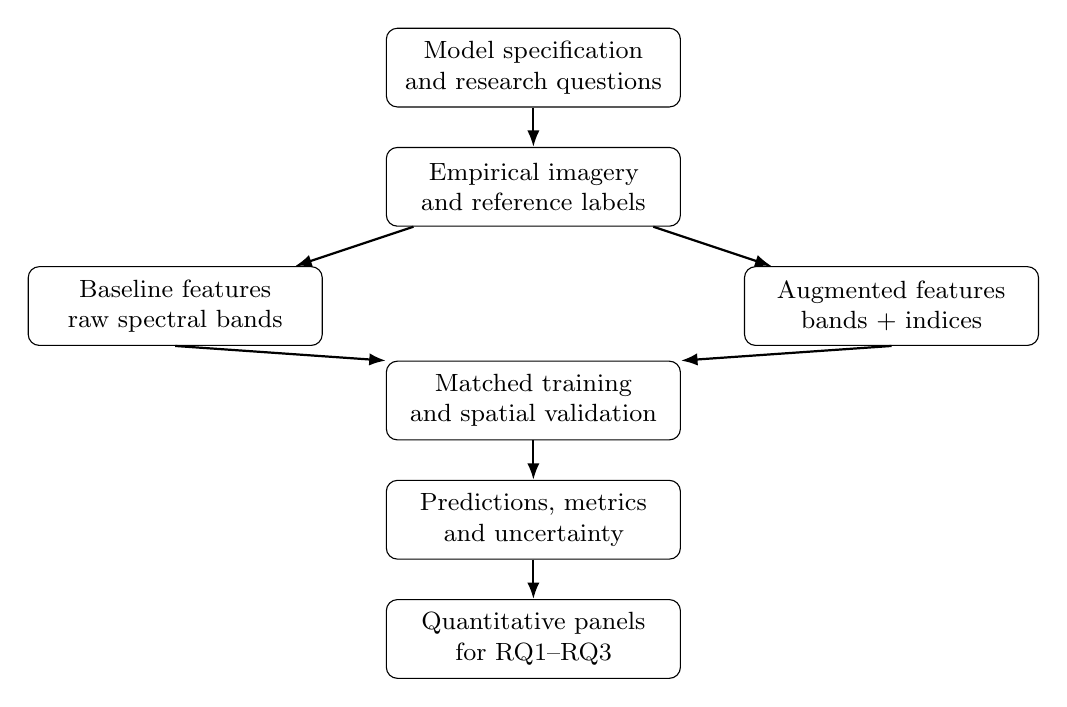
\begin{tikzpicture}[node distance=5mm and 8mm, every node/.style={font=\small},
block/.style={draw,rounded corners,align=center,text width=35mm,minimum height=10mm},
arrow/.style={-{Latex[length=2.1mm]},thick}]
\node[block] (def) {Model specification\\and research questions};
\node[block,below=of def] (inputs) {Empirical imagery\\and reference labels};
\node[block,below left=of inputs] (base) {Baseline features\\raw spectral bands};
\node[block,below right=of inputs] (aug) {Augmented features\\bands + indices};
\node[block,below=17mm of inputs] (train) {Matched training\\and spatial validation};
\node[block,below=of train] (metrics) {Predictions, metrics\\and uncertainty};
\node[block,below=of metrics] (rqs) {Quantitative panels\\for RQ1--RQ3};
\draw[arrow] (def)--(inputs);\draw[arrow] (inputs)--(base);\draw[arrow] (inputs)--(aug);
\draw[arrow] (base.south)--(train.north west);\draw[arrow] (aug.south)--(train.north
east);
\draw[arrow] (train)--(metrics);\draw[arrow] (metrics)--(rqs);
\end{tikzpicture}
\caption{Illustrative workflow. Boxes show theoretical specification,
empirical inputs, matched model comparisons and research question quantitative
outputs.}\label{fig:workflow}
\end{figure}
\subsection{Empirical case study, datasets and parameterization}
\guide{\textbf{This is intentionally the final Method subsection.} Only here identify the
study location, sampling frame, spatial/temporal coverage, named datasets, acquisition
dates, band definitions, labels, coordinate reference system, resolution, preprocessing,
sample counts, missing data procedures, software versions, model parameter values and
access/citation links. Include a study area map if appropriate.}

\section{Results}
\guide{Target ~1,200 words. Structure subsections by RQ if that is the clearest mapping.
Provide multi-panel quantitative graphics with informative captions and consistent scales;
refer to panel (a), (b), etc. Explicitly report \emph{overall magnitude}, \emph{absolute
difference} (including units or percentage points), and \emph{relative difference} (with
reference denominator). Write in dry, neutral terms, which might include little wider explanation, 
no conjecture or advocacy, no literature comparison or causal claims, etc. These belong in Discussion.}
\subsection{RQ1: Baseline performance}
A completed paragraph would report test observations, overall accuracy and class
performance, each keyed to a figure or table. 

You need at least one figure for each RQ, e.g., a panel plot showing overall metrics
with a minimum structre of 2x2 plots.

\subsection{RQ2: Absolute and relative changes}
\fiction\ "Augmented-model accuracy is set to 0.88 (versus 0.83 baseline), a difference of
\textbf{5 percentage points} or approximately \textbf{6.0\% relative to baseline}
($5/83\times100$)". 

\subsection{RQ3: Spatial or subgroup variation}
For this question, compare specific zones, dates, class frequencies, etc., or other predefined
subsets. Give magnitudes and differences. Do not introduce an RQ that the
data cannot answer (this goes back to our discssion on falsifiability).
\begin{figure}[htbp]\centering
\begin{minipage}[t]{0.47\linewidth}\centering\fbox{\parbox[c][1.1in][c]{0.92\linewidth}{\centering\textbf{(a)
Overall performance}\\\small Plot baseline vs. augmented metrics with
intervals}}\end{minipage}\hfill
\begin{minipage}[t]{0.47\linewidth}\centering\fbox{\parbox[c][1.1in][c]{0.92\linewidth}{\centering\textbf{(b)
Absolute / relative changes}\\\small Plot differences; label units and
denominators}}\end{minipage}\\[0.6em]
\begin{minipage}[t]{0.47\linewidth}\centering\fbox{\parbox[c][1.1in][c]{0.92\linewidth}{\centering\textbf{(c)
Per-class metrics}\\\small Precision, recall and F1 by class}}\end{minipage}\hfill
\begin{minipage}[t]{0.47\linewidth}\centering\fbox{\parbox[c][1.1in][c]{0.92\linewidth}{\centering\textbf{(d)
Geographic heterogeneity}\\\small Subgroup or regional variation}}\end{minipage}
\caption{\textbf{Four-panel figure planning guide, not generated results.} Replace each
labeled box with a quantitative plot derived from actual analysis. Specify panels,
samples, metric units, uncertainty, and data sources in the final
caption.}\label{fig:panels}\end{figure}

\section{Discussion}
\guide{Target ~1,100 words. Begin with a quick 1-2 sentence intro (In this section the results are reported by...). 
Then I like to restate the research questions and the purpose of
answering them, so we can systematically address each one by interpreting the evidence for each RQ 
against the literature reviewed in
Section 2. Explain whether results support or challenge prior findings, mechanisms that
could account for patterns (without overstating causality), implications, generalizability
and limitations. Add citations to relevant comparisons. Reserve interpretation for this
section rather than Results.}
\subsection{Revisiting the research questions}
The study set out to answer three questions, including baseline predictive performance (RQ1), the
absolute and relative effect of feature augmentation on measured performance (RQ2), and
variation across subsets (RQ3). 
\fiction\ The demonstration values imply only a hypothetical improvement and cannot
establish a real effect.
\subsection{Interpretation against existing evidence}
Compare actual patterns with the competing claims in the literature. Explain where your findings add an empirical
case, test an existing assumption or produce a methodological contribution. Cite precise
and relevant studies, not simply the same review article in every paragraph.
\subsection{Limitations, implications and next steps}
Assess representativeness, sampling choices, measurement error, label quality,
domain shift, leakage, uncertainty and model assumptions. Separate limitations
that affect internal validity from those affecting generalization. Identify defensible
implications based on the measured evidence and practical next steps.

\section{Conclusion}
\guide{Target ~400 words. \textbf{Open by stating what the paper did and what it
contributes to the literature.} Then give the most important and interesting
\emph{quantitative} findings, with overall values and absolute/relative comparisons where
meaningful. Answer the main RQs directly, and then finish with a concise limitation and
implication for future research. Do not introduce new literature, methods or results, and avoid vague closing
claims.}
This paper has illustrated a framework for testing the incremental predictive performance
of spectral feature engineering in a supervised GeoAI classification system. Its intended
contribution is a transparent comparison of defined feature sets under a common evaluation
design. \fiction\ In the invented example, accuracy increases from 0.83 to 0.88, a
five-percentage-point gain (approximately 6.0\% relative to the baseline). A submitted manuscript must
substitute verified results, explain the contribution in relation to actual published
work, and close with a defensible implication.

\section*{Data and Code Availability}
\guide{Link to real data used, code (e.g., GitHub), reproducible virtual environment, permitted access
restrictions, etc.}\emph{This is a fictional example, so see my published work for examples of real data and code.}
\section*{AI Use and Verification}
\guide{Explain any coding or writing assistance, what was checked independently, and how
you verified citations, results and figures. Follow course policy. I advise you only use it for idea generation, coding, 
grammar/typo checking, etc. (so not writing the actual content, or interpretting content, etc.).}
\begin{thebibliography}{9}
\bibitem[Breiman(2001)]{breiman2001} Breiman, L. (2001). Random Forests. \emph{Machine
Learning}, 45, 5--32.
\bibitem[Belgiu and Drăguț(2016)]{belgiu2016} Belgiu, M. and Drăguț, L. (2016). Random
forest in remote sensing: A review of applications and future directions. \emph{ISPRS
Journal of Photogrammetry and Remote Sensing}, 114, 24--31.
\bibitem[Maxwell et al.(2018)]{maxwell2018} Maxwell, A. E., Warner, T. A., and Fang, F.
(2018). Implementation of machine-learning classification in remote sensing: An applied
review. \emph{International Journal of Remote Sensing}, 39(9), 2784--2817.
\bibitem[Roberts et al.(2017)]{roberts2017} Roberts, D. R. et al. (2017). Cross-validation
strategies for data with temporal, spatial, hierarchical, or phylogenetic structure.
\emph{Ecography}, 40(8), 913--929.
\bibitem[Zhu et al.(2017)]{zhu2017} Zhu, X. X. et al. (2017). Deep Learning in Remote
Sensing: A Comprehensive Review and List of Resources. \emph{IEEE Geoscience and Remote
Sensing Magazine}, 5(4), 8--36.
\end{thebibliography}
\end{document}
